\documentclass[11pt]{article}

\usepackage{amsmath,amsfonts,amssymb}
\usepackage{breqn}
\usepackage[pdftex]{graphicx}
\usepackage{natbib}
\usepackage[usenames,dvipsnames]{xcolor}
%\usepackage[nooneline,tight,raggedright]{subfigure}
\usepackage{multirow}
\usepackage[version=3]{mhchem}

\usepackage{wrapfig}
\usepackage{pstricks,enumerate}
\usepackage{colortbl}
\usepackage{hhtensor}
\usepackage{longtable}
\usepackage[hang,flushmargin,symbol*]{footmisc}
\usepackage[]{algorithm2e}

\usepackage[font=footnotesize,format=plain,labelfont=bf]{caption}
\usepackage{subcaption}

%%%%%%%%% PAGE DIMENSIONS


\setlength{\oddsidemargin}{-0.5in}
\setlength{\textwidth}{5.0in}
\setlength{\topmargin}{-0.5in}
\setlength{\footskip}{0.30in}
\setlength{\textheight}{9.0in}
\setlength{\headheight}{0.2in}
\setlength{\headsep}{0.3in}

%%%%%%%%% SECTIONING STUFF
\makeatletter
\renewcommand{\section}{\@startsection
{section}%
{0}%
{0mm}%
{0.4\baselineskip}%
{0.4\baselineskip}%
{\normalfont\Large\bfseries\color{myBrown}}}%
\makeatother

\makeatletter
\renewcommand{\subsection}{\@startsection
{subsection}%
{1}%
{0mm}%
{0.4\baselineskip}%
{0.4\baselineskip}%
{\normalfont\large\bfseries\color{myBrown}}}%
\makeatother

\makeatletter
\renewcommand{\subsubsection}{\@startsection
{subsubsection}%
{1}%
{0mm}%
{-0.5\baselineskip}%
{0.3\baselineskip}%
{\normalfont\normalsize\itshape\centering\color{myBrown}}}%
\makeatother




\renewcommand{\thesection}{\arabic{section}}
\renewcommand{\thesubsection}{\thesection.\arabic{subsection}}

%\renewcommand*{\thefootnote}{\fnsymbol{footnote}}
%\renewcommand{\footnoterule}{%
%  \kern -3pt
% \hrule width \textwidth height 1pt
%  \kern 2pt
%}

%%%%%%%%% FORMATTING TIDBITS

\definecolor{myTan}{RGB}{205,133,63}
\definecolor{myBrown}{RGB}{155,77,40}
\captionsetup{labelfont={color=myBrown,bf},textfont={color=myTan}}
\newcommand{\HRule}[2]{{\color{myBrown}\rule{#1}{#2}}}
\newcommand{\tPI}[1]{{\color{myBrown}#1}}
\newcommand{\sPI}[1]{\textsc{\color{myBrown}#1}}
\newcommand{\cPI}[1]{\textbf{\color{myBrown}#1}}
\newcommand{\iPI}[1]{\textit{\color{myBrown}#1}}
\newcommand{\lead}[1]{\textit{\color{myBrown}(#1)}}
\newcommand{\tabtit}[1]{\textsc{\color{myBrown}#1}}
\newcommand{\entry}[1]{\mbox{\sffamily\bfseries{#1:}}\hfil}%
\newcommand{\bitem}{\item[{\color{myBrown}$\bullet$}]}
\newcommand{\bmath}{\boldsymbol}
\newcommand{\eps}{\varepsilon}
\newcommand{\Dpartial}[2]{\frac{\partial #1}{\partial #2}}
\newcommand{\itemcolor}[1]{% Update list item colour
\renewcommand{\makelabel}[1]{\color{#1}\hfil ##1}}
\newcommand{\PlasComCM}{\textit{PlasComCM}}
\newcommand{\cl}[1]{\textit{codelet-#1}}
\newcommand{\Cl}[1]{\textit{Codelet-#1}}
\newcommand{\fut}{$^*$}
\newcommand{\pas}{$^\dag$}
\newcommand{\plusplus}[1]{#1{}\texttt{++}}
%%
%%
\newif\ifclean
\cleantrue
%\cleanfalse

%%%%% CONSISTENCY COMMANDS
\newcommand{\eqr}[1]{(\ref{#1})}
\newcommand{\fgr}[1]{figure~\ref{#1}}
\newcommand{\tbr}[1]{Table~\ref{#1}}
\newcommand{\Fgr}[1]{Figure~\ref{#1}}
\newcommand{\secr}[1]{section~\ref{#1}}
\newcommand{\eqnd}[2]{equations~(\ref{#1}) and (\ref{#2})}
\newcommand{\pp}[1]{\ensuremath{\left( #1 \right)}}
\newcommand{\psq}[1]{\ensuremath{{\left[ #1 \right]}}}
\newcommand{\pcrl}[1]{\ensuremath{{\left \{ #1 \right \} }}}
\newcommand{\pang}[1]{\ensuremath{ \left \langle #1 \right \rangle }}
\providecommand{\pop} {}
\renewcommand{\pop}[2] {\ensuremath{\frac {\partial{#1}} {\partial{#2}}} }
\newcommand{\popn}[3] {\ensuremath{\frac {\partial^{#3}{#1}} {\partial{#2}^{#3}}} }
\newcommand{\dod}[2] {\ensuremath{\frac {d{#1}} {d{#2}}} }
\newcommand{\nd}{\ensuremath{~\textrm{and}~}}
\newcommand{\ee}[1]{ \ensuremath{\times 10^{#1}}} 
\newcommand{\plasma}{\ensuremath{\mathrm{c}}}
\newcommand{\plasmar}{\ensuremath{\mathrm{cr}}}
\newcommand{\dancode}{\emph{PlasComCM}}
\newcommand{\bvec}[1]{\ensuremath{\boldsymbol{#1}}}
\newcommand{\mat}[1]{\ensuremath{\mathsf{#1}}}
\newcommand{\parab}[2]{\vspace{#1 pt}\noindent \paragraph{\bf #2 \\}}
\newcommand{\answer}[1]{
$$
\begin{array}{|c|}\hline \\
#1 \\
\\ \hline
  \end{array}
$$}
\newcommand{\Answer}[1]{
\ensuremath{
\begin{array}{|c|}\hline \\
#1 \\
\\ \hline
  \end{array}}}

\DeclareMathOperator\erf{erf}

\usepackage[toc,page]{appendix}
\usepackage{fancyvrb}
% redefine \VerbatimInput
\RecustomVerbatimCommand{\VerbatimInput}{VerbatimInput}%
{fontsize=\tiny,
 %
 frame=lines,  % top and bottom rule only
 framesep=2em, % separation between frame and text
 rulecolor=\color{Gray},
 %
}


%%%%%%%%% COMMENTS/INSTRUCTIONS/NOTES
\setlength{\marginparwidth}{.65in}
\newcommand{\margcomment}[1]{{\color{red}$\bullet$}\marginpar{\raggedright
{\color{red} \tiny #1}}}
\newcommand{\TODO}[1]{{\color{blue}$\bullet$}\marginpar{\raggedright
{\color{blue} \tiny TODO: #1}}}
\usepackage[disable,colorinlistoftodos, color=blue!20!white, bordercolor=gray,
textsize=tiny,textwidth=2.7in]{todonotes}
\newcommand{\LOGM}[1]{\todo[noline,color=green!40]{Luca: #1}}
\newcommand{\LOGF}[1]{\todo[noline,color=orange!40]{JBF: #1}}
\usepackage{color,soul}
\newcommand{\hly}[1]{\textcolor{blue}{#1}}
\usepackage{pstool}
%%%%%%%%%%%%%%%%%%%%%%%%%




%%%%%%%%NOMENCLATURE



%%%% REMOVE COMMENTS
\renewcommand{\hl}{}
\renewcommand{\hly}{}
\setlength{\oddsidemargin}{00.0in}
\setlength{\textwidth}{6.5in}

\begin{document}

\pagestyle{empty}

\begin{center}
\vspace*{1.5in}

\textsc{\color{myBrown} \huge XPACC: PlasCom2 Development Codelets} \\
\bigskip
\cPI{Collaborating authors: {\itshape Daniel Bodony, Michael Campbell}} \\
\medskip
{\color{myTan} The Center for Exascale Simulation of Plasma-Coupled Combustion} \\
{\color{myTan} \textit{University of Illinois at Urbana-Champaign}} \\

\vfil
\begin{minipage}{0.8\textwidth}

The purpose of this document is to describe the codelets used to test the new \dancode-2.0 design.

\end{minipage}

\vfil
\end{center}


\newpage
\setcounter{page}{1}
\pagestyle{plain}


\newpage

\section{Codelet Overview \& Architecture}
The \textbf{XPACC} \textit{PlasCom2} development codelets, \textit{Codelet3} and \textit{Codelet4}, are test and pilot implementations of the planned architecture for the upcoming production version of \textit{PlasCom2}, the next-generation successor to the current \textbf{XPACC} flagship simulation application, \textit{PlasComCM}.  The primary mission for \textit{PlasCom2} development is to provide a platform for physics-based modeling and simulation that is portable and performant on modern (i.e. current and next-generation) high performance computing (HPC) platforms.  The development codelets provide a platform for testing the planned architecture, and programming constructs for use in \textbf{XPACC}-relevant simulations and environments before committing to final design and implementation details.
\begin{wrapfigure}{r}{0.5\textwidth}
\vspace{-20pt}
\begin{center}
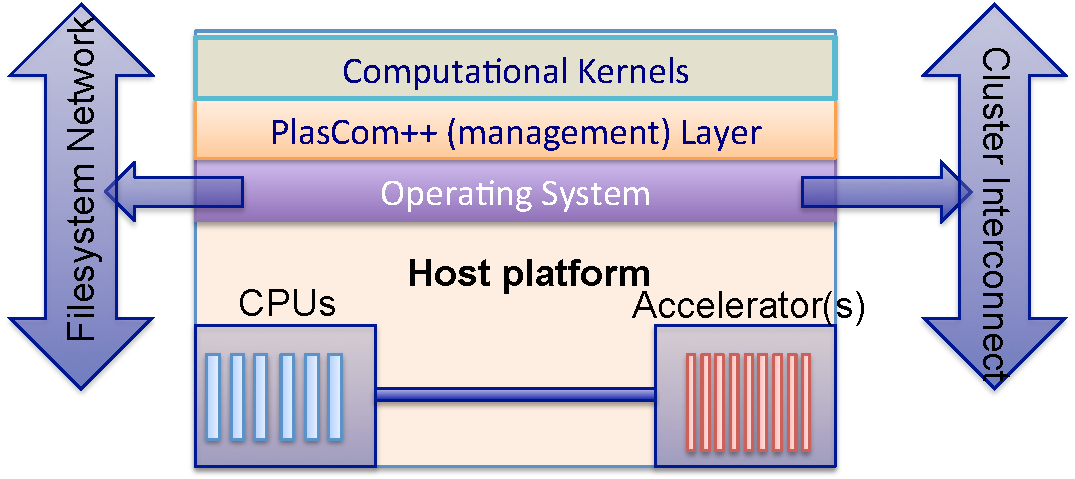
\includegraphics[width=0.48\textwidth]{Figures/HighArch}
\end{center}
\vspace{-20pt}
\caption{Codelet architecture and targeted platform. The typical modern HPC platform consists of a collection of many heterogeneous nodes, each with some number of multi-core host processors, connected by a thin \textit{data straw} to some form of accelerator device with many integrated processing units. The platform OS provides application interfaces to a internode network, and a parallel file system. The codelets are built up from a \plusplus{C} management layer called \plusplus{\textit{PlasCom}} (PCPP), which provides the memory management, I/O, MPI, overall control flow, and other aspects of the parallelism, and a \textit{Kernel} layer which provides focused high-performance numerical operations.}\label{figure:higharch}
\vspace{-10pt}
\end{wrapfigure}

It is expected that the current trend of increasing core-counts and decreasing memory-per-core will continue into the coming generations of HPC platforms. The prototypical platform and general high-level software architecture for the codelets are shown in Figure~\ref{figure:higharch}. The codelets are built-up from a portable, re-usable \plusplus{C} management layer called \plusplus{\textit{PlasCom}} (PCPP), and a \textit{Kernel} layer which provides the focused, high-performance numerical operations. The PCPP layer manages the overall control flow of the simulation application, handles the I/O operations, owns and manages the memory, and manages the parallelism through MPI, OpenMP, and accelerator-targeted language constructs.  The Kernel layer provides high-performance numerical kernels which have extremely limited logic, and operate only on primitive, built-in data types.  Kernel layer constructs are those that are typically transformed, tuned, and targeted for accelerator devices.  Kernels can be written in any language that can be interfaced from \plusplus{C}, but are typically written in Fortran.

There are several design objectives to meet for \textit{PlasCom2} among which are:
\begin{itemize}
\item Drop-in replacement for \textit{PlasComCM}
\item Viable, self-sustainable research tool
\item Demonstrate performance on modern platforms 
\item Address some of the shortcomings of the predecessor codes
\begin{itemize}
\item Performance - I/O, interpolation, general performance on accelerators
\item Overset assembly - needs to be inline, parallel, and dynamic (i.e. support for moving grids)
\item Data structure overhaul - become amenable to CS tool application
\item Repeatability of results
\item Tighter control over development process (w/ testing)
\end{itemize}
\end{itemize}
\section{Software constructs}

\subsection{Simulation}

\subsection{Domain}

\subsection{Grid}

\subsection{State}

\subsection{Advancer}

\subsection{RHS}

\subsection{Kernels}

\section{Codelet Implementation}

\subsection{Partitions and memory buffers}
The following discussion uses integer intervals to describe regions, subregions, and collections (groups) of regions of Cartesian grids, and structured memory buffers. See Appendix~\ref{appendix:intervals} for a brief explanation of intervals the notation used in this document. 

\begin{figure}[h]
\begin{center}
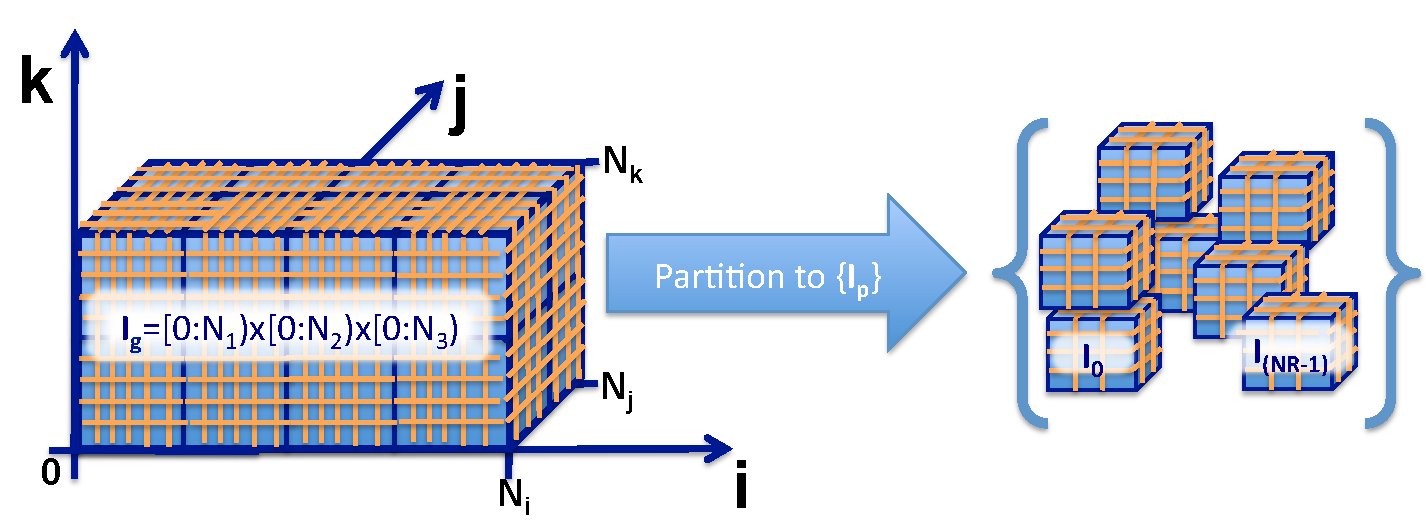
\includegraphics[width=\textwidth]{Figures/Partitions}
\vspace{-20pt}
\caption{Global domain and partitions.}\label{fig:Partitions}
\end{center}
\end{figure}

Given a simulation state with a number $\text{NF}$ of fields, each having a number $\text{NC}_f$ of components each of datatype width $w_f$ bytes, and a single Cartesian grid as shown in Figure~\ref{fig:Partitions} with $\text{N}_1$, $\text{N}_2$, and $\text{N}_3$ points in the computational grid's $\mathbf{\hat{i}}$, $\mathbf{\hat{j}}$, and $\mathbf{\hat{k}}$ directions respectively, and a partitioning or set of $\text{NR}$ non-overlapping partitions $\{\textbf{I}_p\}$ of the overall global grid interval $\textbf{I}_{g}$; the memory buffer constructs and requirements to operate a so-called advancer in the codelets is described. 

\subsubsection{Grid partitions}

As shown in Figure~\ref{fig:Partitions}, the overall global grid interval $\textbf{I}_{g} = [0:\text{N}_1)\times[0:\text{N}_2)\times[0:\text{N}_3)$. Each partition in the group of partitions $\{\textbf{I}_p\}$ (where $0 \leq p < \text{NR}$) is handled by a codelet MPI rank. Strictly speaking, a codelet MPI rank may handle more than one partition, however it is useful for this discussion to assume that there is one partition per MPI rank. The concepts and constructs discussed here easily generalize to the case where there is more than one partition per MPI rank. Assuming the typical situation where there one partition per MPI process, it is instructive to think of the index $p$ in $\{\textbf{I}_p\}$ as denoting the MPI rank of the process that handles a given partition.  Each codelet MPI rank handles a partition with a global interval $\textbf{I}_p = [s_1:e_1]_p\times[s_2:e_2]_p\times[s_3:e_3]_p$, and $(\text{n}_1,\text{n}_2,\text{n}_3)_p$ grid points in each respective dimension, and total number of points $\text{NP}_p = (\text{n}_1 \cdot \text{n}_2 \cdot \text{n}_3)_p$. In the following discussions, when there is little chance of ambiguity, the $p$ subscript is often dropped when referring to partition-local intervals and quantities. Alternatively, $\hat{p}$, is also used to indicate the selection of a single partition.

\subsubsection{Partition halos}

If a given partition's interval $\textbf{I} = [s_1:e_1]\times[s_2:e_2]\times[s_3:e_3]$ does not contain the domain boundary, that is if any of $(s_1,s_2,s_3) \neq (0,0,0)$, or any of $(e_1,e_2,e_3) \neq (\text{N}_1-1,\text{N}_2-1,\text{N}_3-1)$, then some so-called \textit{halo} regions will be required. The halo region itself is an interval that represents a subregion of a partition interval that belongs to a remote MPI process. We refer to the halo region representing a non-local interval as the \textit{remote halo} region, and the subregion of the local interval required by neighboring MPI processes as the \textit{local halo} region.

In particular, if any of $s_i \neq 0$, then the partition is said to have a \textit{left} inter-partition boundary in the $i$ direction (for any $i$ up to number of dimensions of the domain).  If any of $e_i \neq (\text{N}_i-1)$, then the partition is said to have a \textit{right} inter-partition boundary. Otherwise, the partition has a domain boundary in the given direction. The number of points in (or width of) the remote halo region required in the $i$ direction is denoted by $\text{hw}_{i^{-}}$ and $\text{hw}_{i^{+}}$ for the left and right halo regions respectively. These widths are determined independently and subject to constraints imposed by the physics, geometry, and numerical methods used in the simulation.  A two-dimensional example of this situtation is depicted in Figure~\ref{fig:2DPartAndHalos}.

\begin{figure}[h]
\begin{center}
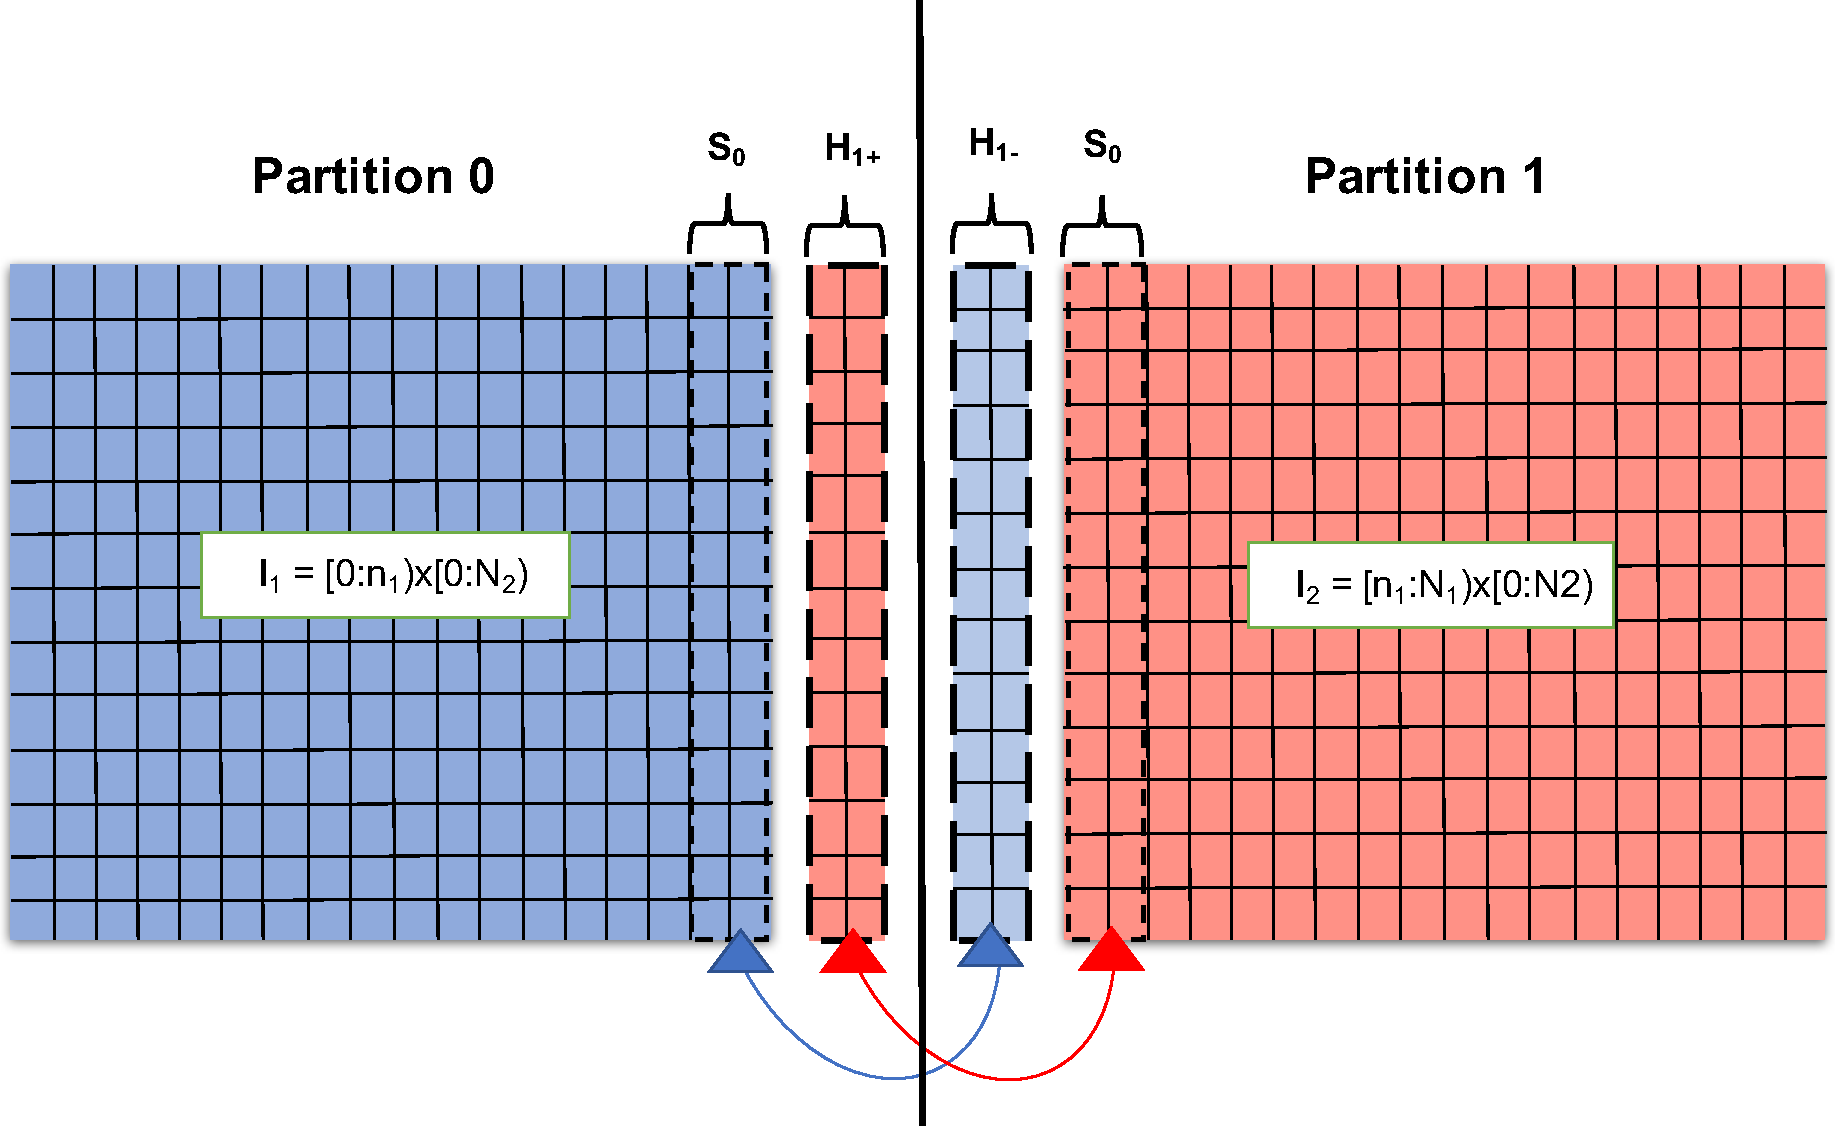
\includegraphics[width=\textwidth]{Figures/PartAndHalos}
\vspace{-20pt}
\caption{2D Partitioning with halos. }\label{fig:2DPartAndHalos}
\end{center}
\end{figure}

\textbf{Remote halo regions} - The collection of required remote halo regions (intervals) $\{\textbf{H}_{i^\pm}\}$ for a given partition are determined by completely local information. For example, in a 3-dimensional domain the halo intervals for the $i=1$ direction are:
 
\begin{equation*} 
\textbf{H}_{1^-} =
\begin{cases}
[(s_1 - \text{hw}_{1^-}):s_1)\times[s_2:e_2]\times[s_3:e_3], & \text{iff}~~s_{1}\neq 0 \\
\emptyset, & \text{otherwise}
\end{cases} 
\end{equation*}
\begin{equation*}
\textbf{H}_{1^+} =
\begin{cases}
(e_1:(e_1 + \text{hw}_{1^+})]\times[s_2:e_2]\times[s_3:e_3], & \text{iff}~~e_{1}\neq (\text{N}_1-1) \\
\emptyset, & \text{otherwise}
\end{cases}
\end{equation*}

These extend in the obvious way to form the halo regions in the other directions. The determination of the partition-local $\text{hw}_{i^{\pm}}$ in each direction $i^{\pm}$ includes consideration of intra-partition boundaries (e.g. objects in the domain), and the data requirements of the numerical methods used in the simulation. It is important to note that a fully local determination of halo requirements can introduce an asymmetry in the inter-partition halo regions, and thus an imbalance in the communication. These potential imbalances can be addressed by overpartitioning.   

\textbf{Local halo regions} - The local halo regions, denoted by $\textbf{S}_h$, indicate the subregion of the local partition interval $\textbf{I}$ that contains data needed by remote processors.   Given the collection of halo intervals from neighboring processors as $\{\{\textbf{H}_{i^{\pm}}\}_h\}$. The local halo regions are found with $\{\textbf{S}_h\} = \textbf{I}\cap\{\{\textbf{H}_{i^{\pm}}\}_h\}~~\forall h\in\{h\}$.

\subsubsection{Partition state buffers}
Each MPI rank creates a set of $\text{NF}$ memory buffers $\{\textit{q}^f_{ijkc}\}$, one for each simulation state field, corresponding to the partition interval, where $0 \leq f < \text{NF}$, and $0 \leq c < \text{NC}_f$, and $0 \leq (i,j,k)< (\text{n}_1,\text{n}_2,\text{n}_3)$.   These are called the \textit{partition state buffers}.  

\begin{figure}[h]
\begin{center}
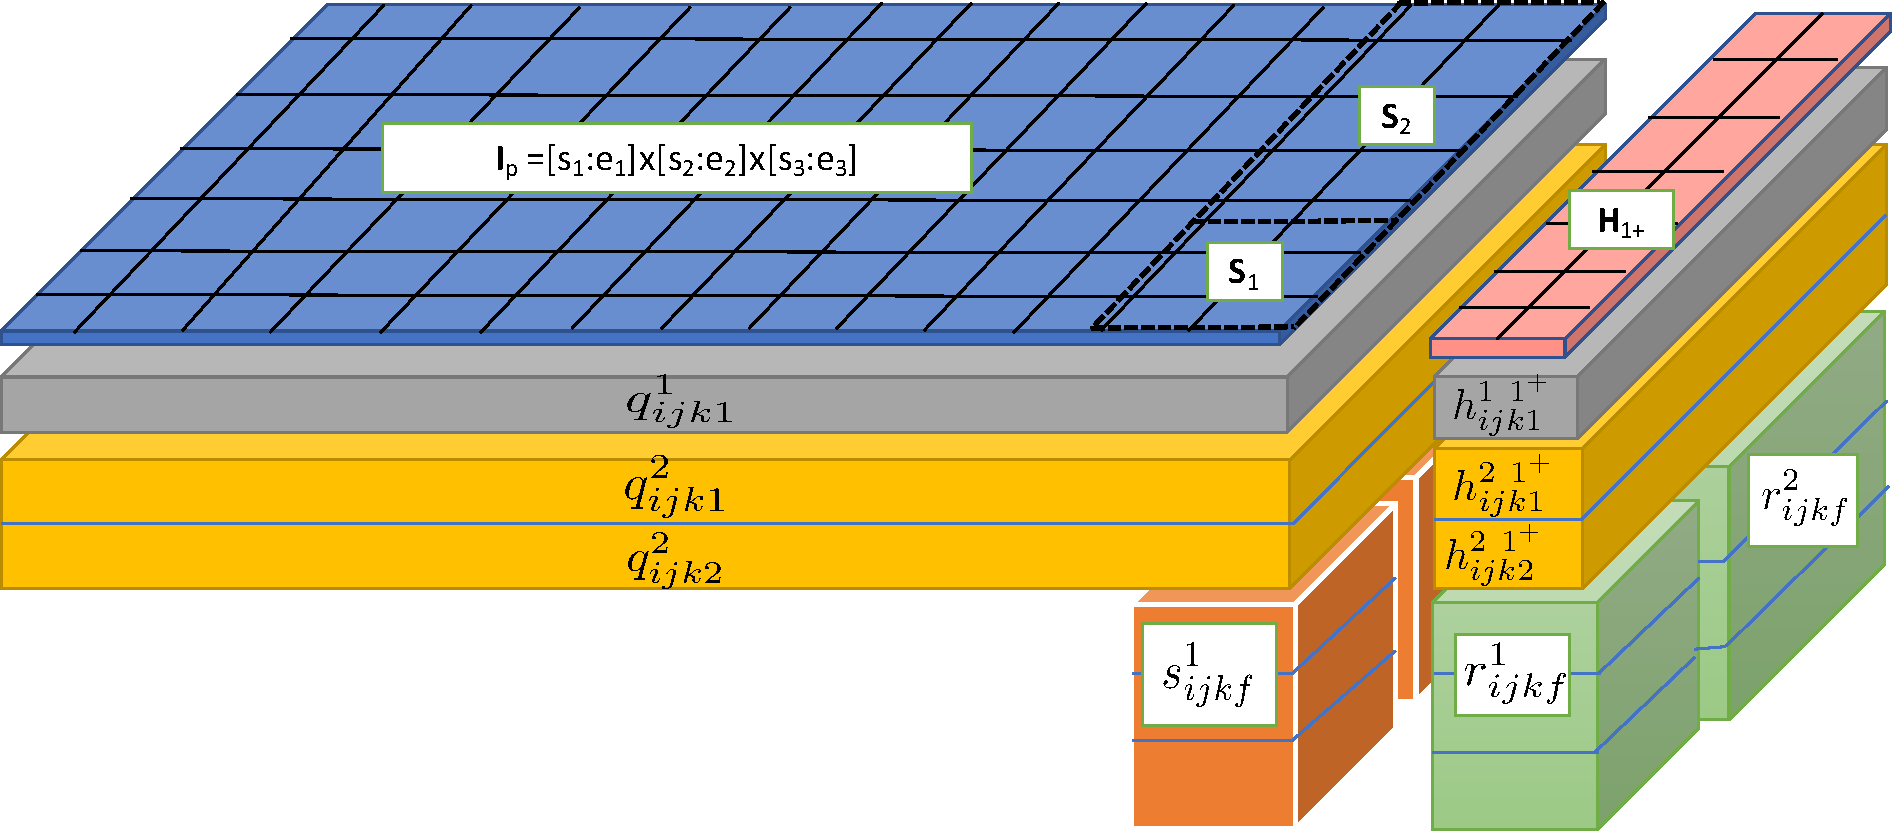
\includegraphics[width=\textwidth]{Figures/PartitionWithBuffers}
\vspace{-20pt}
\caption{Partition with halo and buffers.}\label{fig:Buffers}
\end{center}
\end{figure}

The structure imposed on memory buffers is typically that which corresponds to so-called dictionary ordering wrt $i$, $j$, and $k$. In other words, stride 1 in the $\mathbf{\hat{i}}$ direction, stride $\text{n}_1$ in the $\mathbf{\hat{j}}$ direction, and stride $\text{n}_1 \cdot \text{n}_2$ in the $\mathbf{\hat{k}}$ direction. The ordering of the lower indices in the buffer notation used here is intended to imply the imposed structure, with the inner-most index indicating the stride-1 access.  The upper index ($f$) enumerates the \textit{separate} partition state buffers, i.e. there is a separate partition state buffer for each field.  Note that according to this convention, the partition state buffers are arranged to be contiguous for each field, with a continuous block for each field component.  The general setup for a simulation with two fields (one scalar field, and one two-component vector) is illustrated in Figure~\ref{fig:Buffers}, where the partition state buffer for the scalar field is shown in grey, and the partition state buffer for the two-component vector field is shown in yellow.
 
The number of bytes required to store a single value of a given field is equal to the number of field components times the byte width of the field datatype ($b_f = w_f\cdot\text{NC}_f$). A memory buffer created to hold a point-bound state field in a particular interval of a Cartesian grid must have a size in bytes equal to the number of points in the interval (buffer) times the number of bytes associated with the field, e.g. the total size of each partition state buffer is $\text{NP}_p \cdot b_f$, for each field $f$. 

\subsubsection{Halo and communication buffers}
  Memory buffers will be required to store and communicate the simulation state field values in the halo region. Additionally, some subregion of the local $\textbf{I}$ with supporting buffers will be required for communicating the values of the state fields in the local subregion to the remote MPI process.


\textbf{Remote halo buffers} - A set of memory buffers $\{h^{f d^{\pm}}_{ijkc}\}$, one for each non-empty halo region in each direction $d^\pm$ is created with the same structure as the partition state field buffer, i.e. contiguous for each field, with continuous component blocks, to store the non-local state field data. 

\textbf{Receive buffers} - Having determined the local collection of remote halos $\{\textbf{H}_{i^\pm}\}$, and given the collection of remote partition intervals, $\{\textbf{I}_p\}$, we can determine the collection of global intervals for the receive regions for a particular partition $\hat{p}$, $\{\textbf{R}_h\}_{\hat{p}} = \{\textbf{H}_{i^\pm}\}\cap\{\textbf{I}_p\}~~\forall p\neq \hat{p}$.  The subset of processors (processor ranks) that have non-empty collision intervals with $\{\textbf{H}_{i^\pm}\}$ are referred to as \textit{neighbors}. The collection of all neighbor ranks is called the \textit{neighborhood} and referred to by $\{h\}$. 

$\{\textbf{R}_h\} = [\text{rs}_{h1}:\text{re}_{h1}]\times[\text{rs}_{h2}:\text{re}_{h2}]\times[\text{rs}_{h3}:\text{re}_{h3}]$ represents the global grid intervals on which the state field data values will be received from remote rank $h$. A set of receive buffers, $\{r^h_{ijkf}\}$, one for each neighbor rank $h$ that will send data the local process, are created for storing the communicated data.  Data from the receive buffers is copied into the remote halo buffers for use in computation. Receive buffers are densely packed, i.e. data from all state fields is packed into one buffer, instead of having a separate buffer for each field as is the case for the partition state buffer. 


\textbf{Send buffers} - Send buffers are needed to communicate the state field values in the local halo regions $\{\textbf{S}_h\}$ to the neighboring ranks in $\{h\}$ that need them. The send buffers $\{s^h_{ijkf}\}$ are, like receive buffers, densely packed so that there is one contiguous buffer for all field data, with continuous blocks for each field component. Data are copied from the local halo intervals $\{\textbf{S}_h\} \subset \textbf{I}$ to the send buffers and sent to the neighbor ranks.


\begin{figure}[h]
\begin{center}
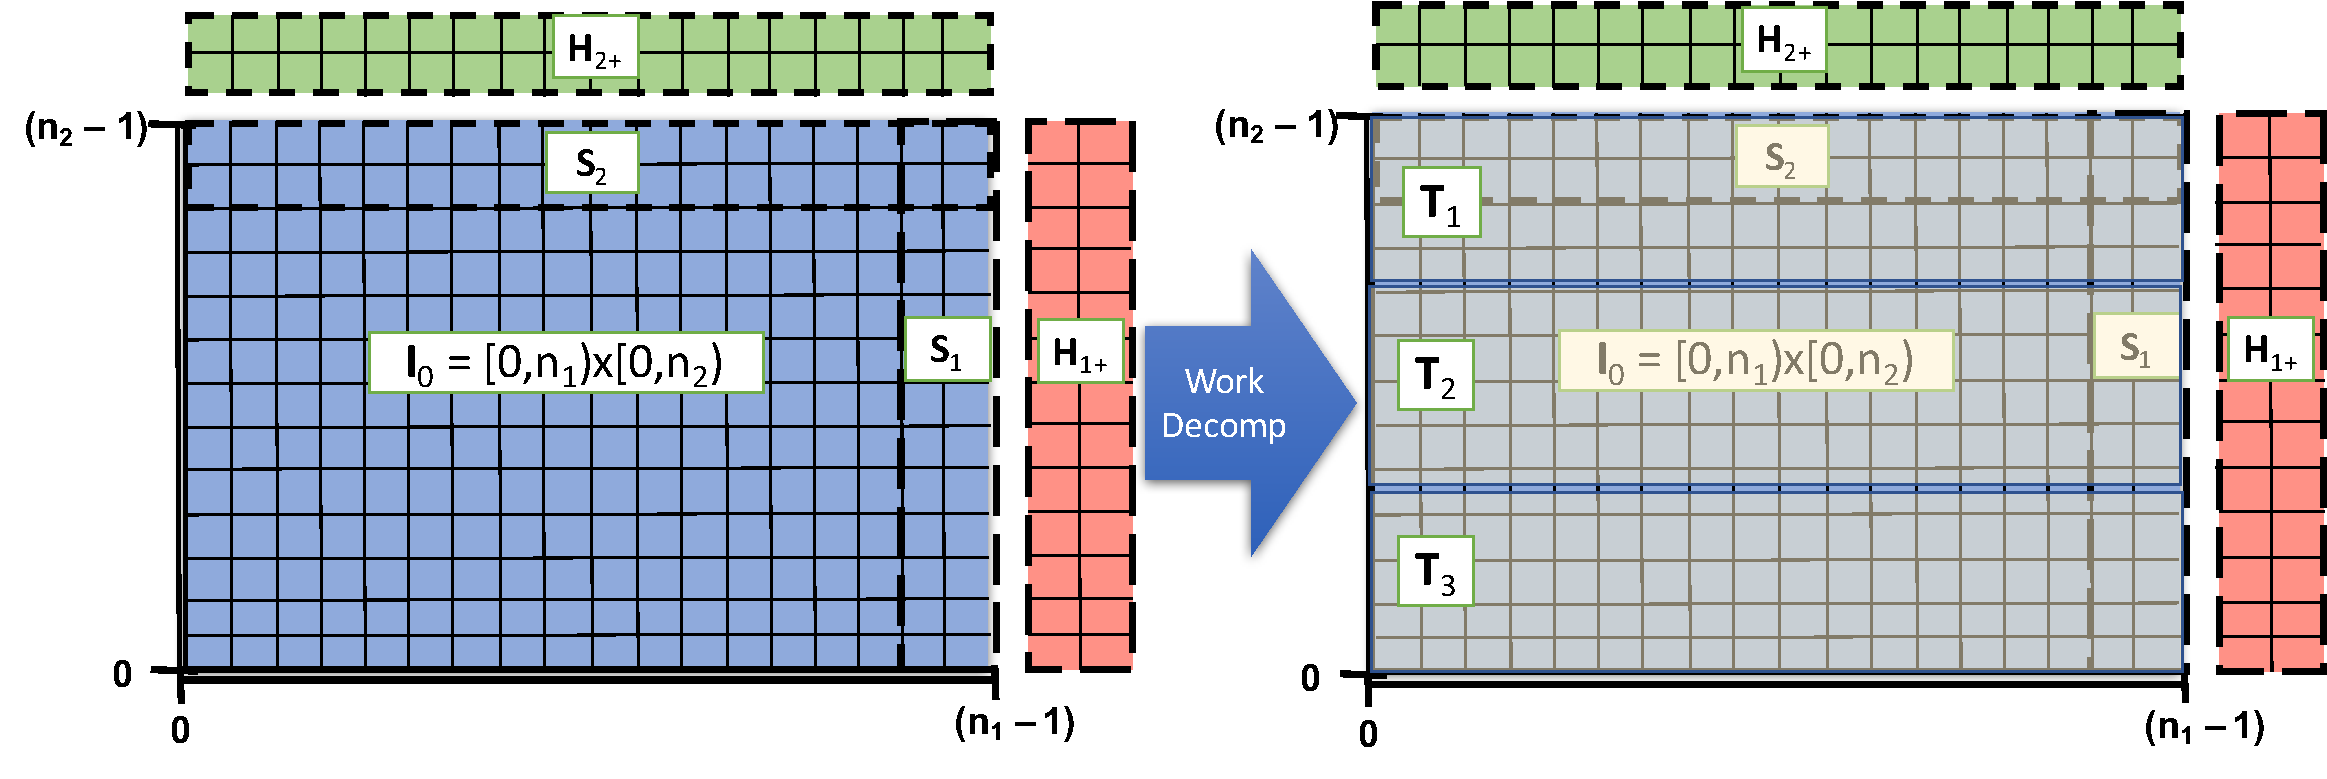
\includegraphics[width=\textwidth]{Figures/WorkDecomp}
\vspace{-20pt}
\caption{Multi-threaded work decomposition.}\label{fig:WorkDecomp}
\end{center}
\end{figure}


\subsection{Advancer}
The proposed software/code construct to implement stepping (e.g. time marching) in \dancode-2.0 is the so-called \textit{Advancer}. The implementation of RK4 stepping in a basic single-grid \textit{Advancer} for \textit{Codelet3} and \textit{Codelet4}  is described as follows.



\newpage
\section{Examples}

\subsection{Advect1D}
The \textit{advect1d} toy code exercises several of the key software constructs and control flows that are planned for \dancode-2.0. 
\subsubsection{Continuous Problem To Be Solved}
We solve the one-dimensional advection equation
\begin{equation}
\frac{\partial u}{\partial t} + \frac{\partial u}{\partial x} = 0, \quad \text{on the domain $\vec{x} \in [0,1]^3, \, t>0$}
\label{eqn:adv}
\end{equation}
subject to the initial and boundary conditions
\begin{equation}
u(\vec{x},0) = u_0(x), \quad u(0,t) = 0.
\label{eqn:bc}
\end{equation}
The general solution is $u(\vec{x},t) = u_0(x - t)$ where we assume that the initial and boundary data are consistent, $u_0(0) = 0$.

\subsubsection{Discrete Problem To Be Solved (1-D Version)}
Ignoring for the moment the three-dimensional domain we introduce ideas in 1-D for simplicity.  We discretize the $x$ domain $[0,1]$ into $\text{N}_1$ grid points with $\text{N}_1-1$ equally spaced intervals of size $\Delta x = 1/(\text{N}_1-1)$.  We label $\bvec{x} = \{x_i\}_{i=1}^{\text{N}_1}$ the discrete points and $\bvec{u} = \{u_i\}_{i=1}^{\text{N}_1}$ the discrete solution on each of the $\text{N}_1$ points.  

We use summation-by-parts (SBP, \cite{strand:1994}) finite difference operators to write the discrete form of $\partial/\partial x$ as $\mat{P}^{-1} \mat{Q}$ where $\mat{P}$ and $\mat{Q}$ have special properties.  To apply the boundary condition $u_1(t) = 0$ we use the simultaneous-approximation-term (SAT, \cite{carpenter/etal:1994}) approach where an additional term proportional to difference of $u_1(t)$ and the boundary data is added to the right-hand-side of the governing equations.

Putting everything together we get the discrete equation to be solved as
\begin{equation}
\frac{\text{d}\bvec{u}}{\text{d}t} + \mat{P}^{-1} \mat{Q} \bvec{u} = -\tau \mat{P}^{-1} \bvec{s} (u_1 - 0), \quad \bvec{u}(0) = \bvec{0},
\label{eqn:discrete}
\end{equation}
where $\tau \ge 1/2$ for numerical stability and $\bvec{s} = [1, 0, \dots, 0]^T$ localizes the boundary condition to the left-most grid point.  Looking at the multiplication $\mat{P}^{-1} \bvec{s}$ shows that, for diagonal $\mat{P}$,
\begin{equation}
\mat{P}^{-1} \bvec{s} = (\mat{P}_{11})^{-1} \bvec{s}.
\end{equation}
There are many SBP operators that are possible but the simplest is the second order scheme
\begin{equation}
\mat{P} = \Delta x \begin{bmatrix} 1 & 0 & 0 & \cdots & 0 & 0 & 0 \\
                                   0 & 2 & 0 & \cdots & 0 & 0 & 0 \\
                                   0 & 0 & 2 & \cdots & 0 & 0 & 0 \\
                                     &   &   & \vdots &   &   &   \\
                                   0 & 0 & 0 & \cdots & 2 & 0 & 0 \\
                                   0 & 0 & 0 & \cdots & 0 & 2 & 0 \\
                                   0 & 0 & 0 & \cdots & 0 & 0 & 1 \end{bmatrix},
\quad
\mat{Q} = \begin{bmatrix} -1 &  1 &  0 & \cdots & 0 & 0 & 0 \\
                          -1 &  0 &  1 & \cdots & 0 & 0 & 0 \\
                           0 & -1 &  0 & \cdots & 0 & 0 & 0 \\
                             &    &    & \vdots &   &   & \\
                           0 &  0 &  0 & \cdots & 0 & -1 & 0 \\
                           0 &  0 &  0 & \cdots & -1 & 0 & 1 \\
                           0 &  0 &  0 & \cdots &  0 & -1 & 1 \\ \end{bmatrix}.
\label{eqn:sbp}
\end{equation}

Equation~(\ref{eqn:discrete}) is of the form
\begin{equation}
\frac{\text{d}\bvec{u}}{\text{d}t} = \bvec{R}(\bvec{u},t)
\label{eqn:eom}
\end{equation}
where $\bvec{R}$ is the right-hand-side vector given by
\begin{equation}
\bvec{R}(\bvec{u},t) = -\mat{P}^{-1} \mat{Q} \bvec{u} - \tau (\mat{P}_{11})^{-1} \bvec{s} (u_1 - 0).
\label{eqn:rhs}
\end{equation}
We choose the Runge-Kutta 4th order time method to integrate Eq.~(\ref{eqn:eom}) in time from an initial state $\bvec{u}(0) = \bvec{0}$.  The full storage form of the RK4 algorithm is

\begin{algorithm}[H]\label{algo:rk4}
\KwData{$N$, $h$, $\bvec{u}_0$, CFL}
$\bvec{u} \leftarrow \bvec{u}_0$\;
$n \leftarrow 1$\;
$t \leftarrow 0$\;
\While{$n \le N$}{
  $\bvec{k}_1 \leftarrow h\bvec{R}(\bvec{u},t)$\;
  $\bvec{k}_2 \leftarrow h\bvec{R}(\bvec{u} + (1/2)\bvec{k}_1,t+(1/2)h)$\;
  $\bvec{k}_3 \leftarrow h\bvec{R}(\bvec{u} + (1/2)\bvec{k}_2,t+(1/2)h)$\;
  $\bvec{k}_4 \leftarrow h\bvec{R}(\bvec{u} + \bvec{k}_3,t+h)$\;
  $\bvec{u} \leftarrow \bvec{u} + (1/6)(\bvec{k}_1 + 2(\bvec{k}_2 + \bvec{k}_3) + \bvec{k}_4)$\;
  $n \leftarrow n + 1$\;
}
\end{algorithm}

\subsubsection{Kernels}
From the algorithm in the previous section there are several possibilities for kernels that could be used.  A simp
le one uses these kernels

\begin{tabular}{ccc}
\textbf{name} & \textbf{input} & \textbf{output} \\
\hline
init & $\bvec{u}_0$, $N$, $\text{N}_1$, CFL & $\bvec{u}$, $\bvec{x}$, $\Delta x$ \\
rhs  & $\bvec{u}$, $h$, $t$ & $\bvec{k}$ \\
rk4  & $\bvec{u}$, $\bvec{k}_1$, $\bvec{k}_2$, $\bvec{k}_3$, $\bvec{k}_4$, $n$ & $\bvec{u}$, $n$ \\
\hline
\end{tabular}

Another possibility splits the rhs into two parts: the interior and BC.  In this case `rhs\_interior' applies $\mat{P}^{-1}\mat{Q}$ to $\bvec{u}$ while `rhs\_bc' applies $-\tau (\mat{P}_{11}^{-1}) \bvec{s}$.

\newpage

\appendix

\section{Integer intervals and partitions}\label{appendix:intervals}

To effectively discuss details about software constructs for grid and buffer handling in the codelets, some language, conventions, and notions about integer intervals and their interactions need to be developed. 

We consider domains discretized by collections of uniform $n$-dimensional Cartesian grids with a number of points $\text{N}_1$, $\text{N}_2$, and $\text{N}_3$ in the $\mathbf{\hat{i}}$, $\mathbf{\hat{j}}$, and $\mathbf{\hat{k}}$ directions respectively along with a curvilinear mapping  from the Cartesian computational coordinates ($\chi$, $\xi$, $\eta$) to physical coordinates ($x$, $y$, $z$) and its Jacobian $\frac{\partial(\chi,\xi,\eta)}{\partial(x,y,z)}$. 

Regions and subregions of the discrete computational domain can be represented by intervals (or pairs of numbers) in the $n$-dimensional space of positive integers, i.e. $\textbf{I}\in\mathbb{Z^+}^{2n}$. In this document, a notation semi-consistent with programming languages and constructs will be used wherein $[a:b]$ represents the closed interval $[a, a+1, ..., b]$, $[a:b)$ represents the closed interval $[a, a+1, ..., b-1]$, and $(a:b]$ represents the closed interval $[a+1, a+2, ..., b]$, where $a,b\in\mathbb{Z^+}$. A region or interval, $\textbf{I}$ of the $n$-dimensional computational space is then described by the Cartesian product of $n$ such intervals, e.g. in 3 dimensions, $\textbf{I} = \textbf{I}_1\times\textbf{I}_2\times\textbf{I}_3$.   

An unpartitioned Cartesian grid having $\text{N}_1$, $\text{N}_2$, and $\text{N}_3$ points in the $\mathbf{\hat{i}}$, $\mathbf{\hat{j}}$, and $\mathbf{\hat{k}}$ directions, respectively has the \textit{global} grid interval, $\textbf{I}_{g} = [0:\text{N}_1)\times[0:\text{N}_2)\times[0:\text{N}_3)$. A one-dimensional grid interval $\textbf{I} = [s:e]$ has a number of points $\text{n} = e - s + 1$, and an $n$-dimensional interval $\textbf{I} = [s_1:e_1]\times[s_2:e_2]\times...\times[s_n:e_n]$ has a number of points $\text{NP} = \prod_{i=1}^{n} (e_i - s_i + 1)$. An empty or null interval has $0$ points and is denoted by $\mathbf{\emptyset}$.

A partition or subregion of a 3-dimensional Cartesian grid, for example,  is a partition interval $\textbf{I}_{p} = [s_1:e_1]\times[s_2:e_2]\times[s_3:e_3]~~\forall~ s_i \leq e_i < \text{N}_i$. The intersection (or overlap) of two one-dimensional intervals is described as follows.
\begin{equation} 
\textbf{I}_{1}\cap\textbf{I}_{2} =
\begin{cases}
[\max_{}(s_1,s_2),\min_{}(e_1,e_2)], & \text{iff}~~s_{2}\geq e_{1}$ \text{and} $s_{1} \leq e_{2} \\
\emptyset, & \text{otherwise}
\end{cases}
\end{equation}

The intersection of two n-dimensional intervals, $\textbf{I} = \textbf{I}_{1}\times\textbf{I}_{2}\times...\times\textbf{I}_{n}$ and $\textbf{J} = \textbf{J}_{1}\times\textbf{J}_{2}\times...\times\textbf{J}_{n}$ is defined as follows.

\begin{equation}                                                                                                  
\textbf{I}\cap\textbf{J} =                                                                               
\begin{cases}                                                                                                     
(\textbf{I}_{1}\cap\textbf{J}_{1})\times(\textbf{I}_{2}\cap\textbf{J}_{2})\times...\times\textbf{I}_{n}\cap\textbf{J}_{n}, & \text{iff}~~\textbf{I}_{i}\cap\textbf{J}_{i}\neq\emptyset~~\forall~i\leq n\\                
\emptyset, & \text{otherwise}                                                                                     
\end{cases}                                                                                                       
\end{equation}

Intervals that do not overlap or intersect are said to be \textit{disjoint}. Sets or collections of intervals are denoted by $\{\textbf{I}_1,\textbf{I}_2,...,\textbf{I}_m\}$ or simply $\{\textbf{I}_{i}\}$. A set of intervals $\{\textbf{I}_i\}$ is said to be mutually disjoint if $\textbf{I}_i\cap\textbf{I}_j = \emptyset~~\forall~i\neq j$. Formally, a \textit{partitioning} of $\textbf{I}_{g}$ is a set of non-empty mutually disjoint intervals $\{\textbf{I}_{p}\}$, wherein $\cup\{\textbf{I}_{p}\} = \textbf{I}_{g}$. Informally, we say that our Cartesian grid is partitioned into a set of $\text{NR}$ non-overlapping regions (partitions) $\{\textbf{I}_{p}\}$ which cover the grid. 

\newpage

\section{Questions}

If $\bvec{R}(\bvec{u},t)$ is a linear mapping, then $\bvec{R}(\bvec{u}+\bvec{v},t) = \bvec{R}(\bvec{u},t) + \bvec{R}(\bvec{v},t)$, and $\bvec{R}(\alpha\bvec{u},t) = \alpha\bvec{R}(\bvec{u},t)$. Expanding out the RK4 algorithm above:\\

$\bvec{k}_2 \leftarrow h\bvec{R}(\bvec{u}+(1/2)\bvec{k}_1) = h\bvec{R}(\bvec{u}) + (h^2/2)\bvec{R}(\bvec{R}(\bvec{u})) = h\bvec{R}(\bvec{u}) + (h^2/2)\bvec{R}^2(\bvec{u})$ \\

$\bvec{k}_3 \leftarrow h\bvec{R}(\bvec{u}+(1/2)\bvec{k}_2) = 
h\bvec{R}(\bvec{u}) + (h/2)(\bvec{R}(h\bvec{R}(\bvec{u}) + (h^2/2)\bvec{R}^2(\bvec{u}))) \\ \hspace{\fill}
= h\bvec{R}(\bvec{u}) + (h^2/2)\bvec{R}^2(\bvec{u}) + (h^3/4)\bvec{R}^3(\bvec{u})$ \\

$\bvec{k}_4 \leftarrow h\bvec{R}(\bvec{u} + \bvec{k}_3) = h\bvec{R}(\bvec{u}) + h\bvec{R}(h\bvec{R}(\bvec{u}) + (h^2/2)\bvec{R}^2(\bvec{u}) + (h^3/4)\bvec{R}^3(\bvec{u})) = \\
= h\bvec{R}(\bvec{u}) + h^2\bvec{R}^2(\bvec{u}) + (h^3/4)\bvec{R}^3(\bvec{u}) + (h^4/4)\bvec{R}^4(\bvec{u})$ \\

$\bvec{u}(t+\Delta{t}) = \bvec{u}(t) + (1/6)(\bvec{k}_1 + 2(\bvec{k}_2 + \bvec{k}_3) + \bvec{k}_4) = \\
\bvec{u}(t) + h\bvec{R}(\bvec{u}(t)) + (h^2/2)\bvec{R}^2(\bvec{u}(t)) + (h^3/6)\bvec{R}^3(\bvec{u}(t)) + (h^4/24)\bvec{R}^4(\bvec{u}(t))$

This matches the Taylor expansion for a function, $\bvec{f}(t+\Delta{t})$ for small $\Delta{t}$; i.e.:\\


$\bvec{f}(t+\Delta{t}) \approx \bvec{f}(t) + \Delta{t}\frac{d\bvec{f}}{dt} + ({\Delta{t}}^2/2)\frac{d^2\bvec{f}}{dt^2} + ({\Delta{t}}^3/6)\frac{d^3\bvec{f}}{dt^3} + ({\Delta{t}}^4/24)\frac{d^4\bvec{f}}{dt^4} + O({\Delta{t}}^5)$


\newpage
\bibliographystyle{jfm}
\bibliography{references}

\newpage

\subsection*{Acknowledgment}

This material is based in part upon work supported by the Department
of Energy, National Nuclear Security Administration, under Award
Number DE-NA0002374.

\subsection*{Disclaimer}

This report was prepared as an account of work sponsored
by an agency of the United States Government. Neither the United
States Government nor any agency thereof, nor any of their
employees, makes any warranty, express or implied, or assumes any
legal liability or responsibility for the accuracy, completeness, or
usefulness of any information, apparatus, product, or process
disclosed, or represents that its use would not infringe privately
owned rights. Reference herein to any specific commercial
product, process, or service by trade name, trademark, manufacturer,
or otherwise does not necessarily constitute or imply its endorsement,
recommendation, or favoring by the United States Government or any
agency thereof.  The views and opinions of authors expressed herein do
not necessarily state or reflect those of the United States Government
or any agency thereof.


\end{document}
%-------------------------------------------------------------------------
